\documentclass{article}

\usepackage[paper=letterpaper,margin=2.5cm]{geometry} % Set Margins

%% Math and math fonts
\usepackage{amsthm, amssymb, amsfonts, amsmath}
\usepackage{bbm} % for \mathbbm{1}

% date
\usepackage[nodayofweek]{datetime}

% Color
\usepackage{color, xcolor}

% Misc
\usepackage{environ}  % \collect@body in asmmath
\usepackage{graphicx} % \includegraphics options
\usepackage{mdframed} % text boxes
\usepackage{indentfirst} % Indent first paragraph after section header
\usepackage[shortlabels]{enumitem} % Control enumerate items with [(a)]
\usepackage{comment} % Comments
\usepackage{fancyhdr} % Headers and footers

% Tables
\usepackage{array}

% Sub-figures and figure placement
\usepackage{caption}
\usepackage{subcaption}
\usepackage{float} 

% Graphing
\usepackage{pgfplots}
\pgfplotsset{compat=1.17}
\usepackage{tikz}

% Title Placement
\usepackage{titling}
\setlength{\droptitle}{-6em}

%set indent to 
\setlength{\parindent}{0pt}

% Hyper refs
\usepackage{hyperref}
\hypersetup{
    colorlinks=true,
    linkcolor=blue,
    urlcolor  = blue,
    filecolor=magenta,      
    urlcolor=blue,
    citecolor = blue,
    anchorcolor = blue
}

% % Citation management
\usepackage{natbib}
\bibliographystyle{abbrvnat}
\setcitestyle{authordate,open={(},close={)}}

\pagestyle{fancy}

\usepackage[paper=letterpaper,margin=2.5cm]{geometry} % Set Margins

%% Math and math fonts
\usepackage{amsmath, amsthm, amssymb, amsfonts}
\usepackage{bbm} % for \mathbbm{1}

% date
\usepackage[nodayofweek]{datetime}

% Color
\usepackage{color, xcolor}

% Misc
\usepackage{environ}  % \collect@body in asmmath
\usepackage{graphicx} % \includegraphics options
\usepackage{mdframed} % text boxes
\usepackage{indentfirst} % Indent first paragraph after section header
%\usepackage[shortlabels]{enumitem} % Control enumerate items with [(a)]
\usepackage{comment} % Comments
\usepackage{fancyhdr} % Headers and footers

% Tables
\usepackage{array}

% Sub-figures and figure placement
\usepackage{caption}
\usepackage{subcaption}
\usepackage{float} 

% Graphing
\usepackage{pgfplots}
\pgfplotsset{compat=1.17}
\usepackage{tikz}

% Title Placement
\usepackage{titling}
\setlength{\droptitle}{-6em}

%set indent to 
\setlength{\parindent}{0pt}

% Hyper refs
\usepackage{hyperref}
\hypersetup{
    colorlinks=true,
    linkcolor=blue,
    urlcolor  = blue,
    filecolor=magenta,      
    urlcolor=blue,
    citecolor = blue,
    anchorcolor = blue
}

% % Citation management
\usepackage{natbib}
\bibliographystyle{abbrvnat}
\setcitestyle{authordate,open={(},close={)}}

% ----------------------------------------
% TITLE
% ----------------------------------------

\pagestyle{fancy}

\lhead{Creel}
\chead{More Integrals}
\rhead{AMES}

\title{AMES Class Notes -- Week Six, Day 2: More integrals}
\author{Andie Creel}

\begin{document}
\maketitle

\section{Finishing "Additively Separable" Ex. from Monday}

In this example, we will see how the constants from separate terms of the integral can be combined into one final constant. \\

Consider the function 
\begin{align}
    f(x) = \int 7x^2 + 3x +6 dx.
\end{align}

The integral is a "linear operator" so we can integrate each of these terms that are separated by addition signs separately, 

\begin{align}
    f(x) = \int 7x^2 dx + \int 3x dx +\int 6dx.
\end{align}
We can now use the integral's version of the power rule to integrate these. \\

\textbf{Integral power rule:}

\begin{align}
    \int x^n dx = \frac{1}{n}x^{n+1} + C
\end{align}

applying the power rule to each term gives us 
\begin{align}
    f(x) = (\frac{7}{3} x^3 + X) + (\frac{3}{2} x^2 + Y) + (6x + Z) \label{consts}
\end{align}
where $X, Y, Z$ are our unknown constants. We can define another unknown constant as 
\begin{align}
    C = X + Y + Z 
\end{align}
and rewrite \ref{consts} as 
\begin{align}
    f(x) = \frac{7}{3} x^3  + \frac{3}{2} x^2 + 6x + C. 
\end{align}

This shows us that even though each separate term we're integrating may have it's own constant, we can combine them into a single final constant during integration. 


\section{Integration by U-substitution}

\begin{align}
    \int f(u) \frac{du}{dx}dx = \int f(u) du
\end{align}

\textbf{Example}
\begin{align}
    f(x) = \int x e^{x^2} dx
\end{align}
Let $u = x^2$, $du = 2x dx$, $\frac{du}{2x} = dx$
\begin{align}
   &= \int e^{x^2} x dx \\
    &= \int \frac{e^u}{2}du \\
    &= \frac{1}{2} \int e^u du \\
    &= \frac{1}{2} e^u \\
    &= \frac{1}{2} e^{x^2}
\end{align}



\section{The importance of discounting: $e^{-rt}$}


Consider a funny integral: 
\begin{align}
    \int_0^\infty e^{-rt}dt
\end{align}
Why is this weird? Because the support is 0 to $\infty$. However, when we integrate it, we will see that the area under this curve is finite (despite the function going to infinity). Let's show this is true with a U-sub. \\

Let 
\begin{align}
    U = -rt \label{U}\\
    \frac{dU}{dt} = -r \implies \\
    dU = -r dt \implies \\
    \frac{dU}{-r} = dt \label{dt}
\end{align}

plug in \ref{U} and \ref{dt} into our original integral 
\begin{align}
    &= \int_0^\infty - \frac{1}{r} e^U du\\
    &= -\frac{1}{r} \int_0^\infty e^u du\\
    &= -\frac{1}{r} e^u \bigg|_0^\infty \\
    &= -\frac{1}{r} e^{-rt} \bigg|_0^\infty \\
    &=  -\frac{1}{r} e^{-r\infty} - -\frac{1}{r} e^{-r 0} \\
    &= \frac{1}{r} ( -e ^{-r\infty} + e^{-r0} \\
    &= \frac{1}{r} (0 + 1) \\
    &= \frac{1}{r}
\end{align}

Even though we integrated over an infinite support (0 to $\infty$) we have a finite area. \\

This is \textbf{exponential decay} or a \textbf{discounting process}. This is a very important integral and it's used in applied settings often. \\

This discount factor means that we can project a program into the future \textit{infinitely} and still find a finite value for the impact of that program. We can compare a program from now to the end of the world to a another program for the same length of time and see how they differ. \\

For example:
\begin{align}
    X = \int_0^\infty M(t) e^{-rt} dt\\
    Y = \int_0^\infty N(t) e^{-rt} dt
\end{align}

We can compare $X$ and $Y$ over an arbitrarily long period. If $M(t)$ represented a policy that affected wellbeing, and $N(t)$ was an alternative policy, we could use the discount rate $e^{-rt}$ to be able to evaluate which of those programs would achieve sustainable development goals over an arbitrarily long period.\\

\subsection{Thin and Fat Tails}


\begin{figure}[htp]
    \centering
        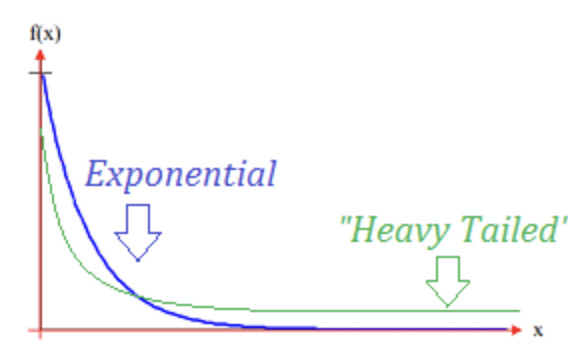
\includegraphics[width=0.5\textwidth]{Screen Shot 2023-10-04 at 10.56.06 AM.png}
    \caption{https://www.statisticshowto.com/fat-tail-distribution/}
    % \label{fig:sample}
\end{figure}

Above, if you were to integrate the "heavy tail" function it would not be finite! As x goes to $\infty$ the area under the function keeps getting bigger and bigger. If you were to integrate the "heavy tailed" function it would "blow up" aka go to infinity. \\

The if you were to integrate under the "exponential" function in the picture above, you would get a finite answer similar to the function $e^{-rt}$. \\

\section{Integration by parts}
It's not as bad as you think it is! Previously, integration by substitution is similar to the chain rule for derivatives. Integration by parts is \textit{kind of} like the product rule for derivatives. \\

Integration by parts is not really an integral trick, it's more like an algebra trick. \\

Consider the function 
\begin{align}
    z(x) = f(x) g(x)
\end{align}

We want the integral of $z(x)$ 
\begin{align}
    Z(x) = \int f(x)g(x) dx 
\end{align}

Now, we know how to get $dz(x) /dx$ using the product rule
\begin{align}
    \frac{dz(x)}{dx} = f'(x) g(x) + f(x) g'(x) \implies\\
    \int dz = \int (f'(x) g(x) + f(x) g'(x)) dx 
\end{align}

Remember integrals are linear operators
\begin{align}
    \int dz = \int f'(x) g(x) dx + \int f(x) g'(x) dx\\
\end{align}
Note that $\int dz = z(x) = f(x) g(x)$
\begin{align}
    f(x) g(x) = \int f'(x) g(x) dx + \int f(x) g'(x) dx \implies \\
    f(x) g(x) - \int f(x) g'(x) dx = \int f'(x) g(x) dx \\
    f(x) g(x) - \int f(x) g'(x) dx = \int g(x) f'(x) dx  \\
    \int g(x) f'(x) dx = f(x) g(x) - \int f(x) g'(x) dx
\end{align}

Let 
\begin{align}
    U = g(x) \\
    dV = f'(x)dx \\
    V = f(x) \\
    dU = g'(x)dx
\end{align}
Plug these back into our last equation 

\begin{align}
    \int U dV = V U - \int V dU
\end{align}
which is the equation for integration by parts. \\

Here's an example. Consider the function $A(x)B(x)$ 
\begin{align}
    \int A(x) B(x)dx = A(x) \int B(x) dx - \int A(x) \frac{d B(x)}{dx} dx
\end{align}
We've set: 
\begin{align}
    dV = B(x)dx \implies\\
    V = \int B(x) dx
\end{align}
which is why we have $\int B(x) x$ is in the first term of the right hand side.

\subsection{Tips}
How can you remamber the order of what should be U and what should be dV? \\
U $\rightarrow$ Log $\rightarrow$ Inverse trig $\rightarrow$ Algebraic $\rightarrow$ Trig $\rightarrow$ Exponential $\rightarrow$ dV \\


\subsection{Example}
Consider the function 
\begin{align}
    \int x  e^x dx
\end{align}

Whats's U and what's V? 
\begin{align}
    \int U dV = vu - \int V dU\\
    U = x\\
    dU = dx \\
    V = e^x\\
    dV = e^x dx
\end{align}

Rewrite the whole thing! And use integration by parts
\begin{align}
    \int x e^x dx &= e^x x - \int e^x dx \\
    &= e e^x - e^x \\
    &= (x - 1) e^x
\end{align}


\section{Integrating logs}

Consider 
\begin{align}
    \int \frac{dx}{x} = \int \frac{1}{x} dx = ln(x)
\end{align}
Cool! Wait, but what about
\begin{align}
    \int ln(x) dx = ??
\end{align}
This was a really hard problem that existed for a very long time in mathematics. What's the trick? Consider this function instead 

\begin{align}
    \int ln(x) 1 dx 
\end{align}
Now we can use integration by parts.

\begin{align}
    U = ln(x) \\
    dU = \frac{1}{x} dx\\
    V = x \\
    dV = 1 dx\\
\end{align}
\textbf{Do NOT forget the $dx$ when you get $dU$!!} Now, plug it all back into our integration by parts formal 
\begin{align}
    \int U dV &= V U - \int V dU\\
    \int ln(x) 1 dx &= x ln(x) - \int x \frac{1}{x} dx \implies \\
    &= x ln(x) - \int 1 dx  \\
    & = x ln(x) - x\\
    &= x (ln(x) - 1)
\end{align}
You can take the derivative of this final equation to check and you'll find the derivative of that final equation does equal $ln(x)$.

\section{Double Integral}
We need to sum over one variable and then we sum over the other.
\begin{align}
    \int \int xy dx dy = \int \bigg(\int xy dx\bigg) dy 
\end{align}
We can solve the integral in parentheses first while treating $y$ like a constant 
\begin{align}
    &= \int \bigg( y\int x dx\bigg) dy \\
    &= \int \bigg( y\frac{1}{2} x^2 \bigg) dy
\end{align}
Now we can treat $x$ as a constant
\begin{align}
    &= \frac{1}{2} x^2 \int y dy\\
    & = \frac{1}{2} x^2 * \frac{1}{2} y^2 + C\\
    &= \frac{1}{4} x^2 y^2 + C
\end{align}







\end{document}